\chapter{Experimental Setup and Results}

\section{Laser System}
\begin{figure}
  \begin{center}
    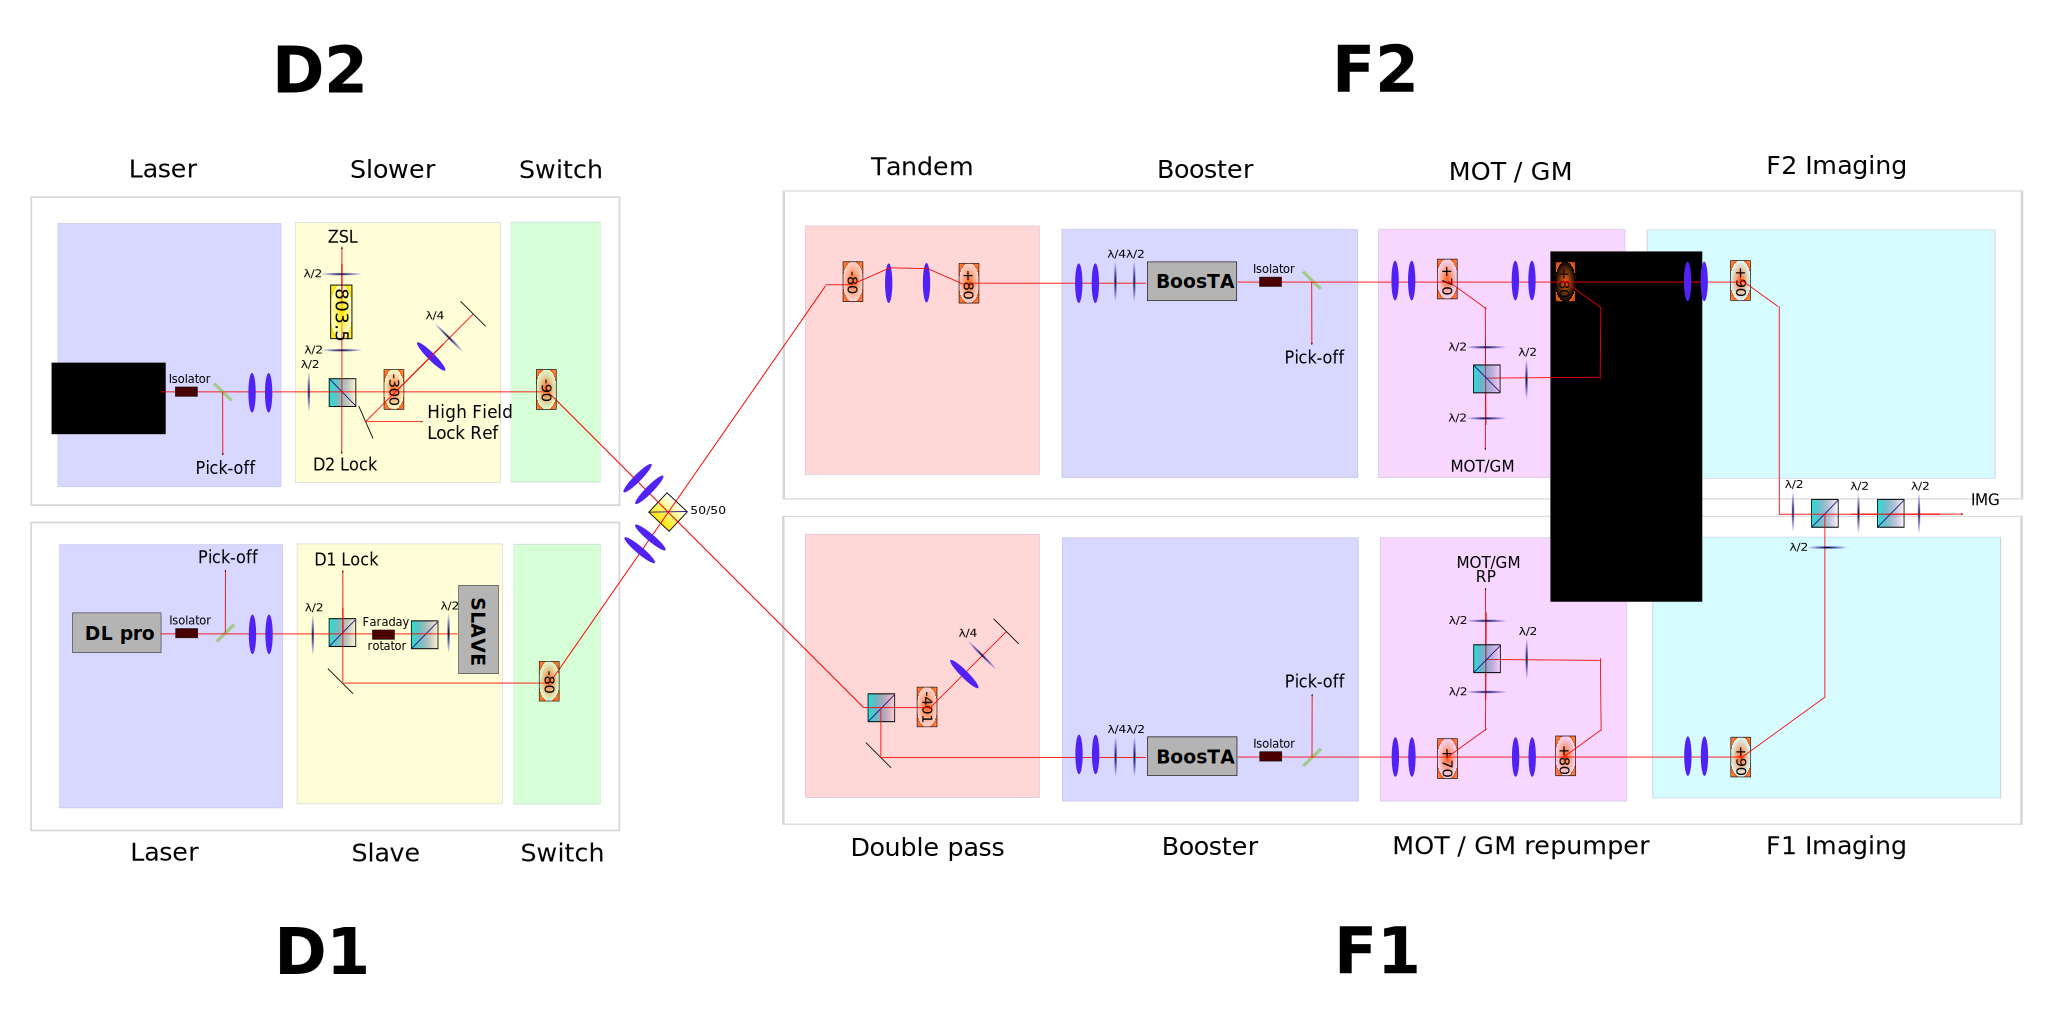
\includegraphics[width=10cm]{laser_table.png}
  \end{center}
  \caption{Schematic of the laser table design}
  \label{laser-table}
\end{figure}

\section{Vacuum Chamber and Main Coils Configuration}

\section{Spin Flip Zeeman Slower}

\section{Magneto-Optical Trap (MOT) and Compressed-MOT}

CMOT

\section{Gray Molasses}

\section{Dark State Pumping}

At the end of Laser cooling, the atoms are distributed in different ground states.\\
In order to trap in MT, need to go to 2, 2 / 2, 1 which are the only trappable states at both low field and high field.\\
Choose 2, 2 because we can use dark state pumping which ...

Dark State pumping with D1 light

Re-scattering, detuning

\section{Static Magnetic Trap}

\section{Optical Dipole Trap}

\section{Bose-Einstein Condensate}
